%\documentclass[aspectratio=43,12pt]{beamer}
%\beamertemplatenavigationsymbolsempty

\usepackage{helvet}
\usepackage{times}

\usefonttheme[stillsansseriflarge]{serif}
\usecolortheme{dove}


\documentclass[12pt,twocolumn]{article}
\usepackage{beamerarticle}
\usepackage{amsmath}

\usepackage{times}
\usepackage{helvet}

%\usepackage{fontspec}
%\setmainfont{Liberation Serif}
%\setsansfont{Liberation Sans}

\usepackage{geometry}
\geometry{               
	letterpaper,
	bottom=0.5in,
	top=0.5in,
	inner=1in,
	outer=0.5in,
        footskip=4ex
}

\usepackage{graphicx}

%\usepackage{titling}
%\pretitle{\begin{center}\LARGE\sffamily}
%\posttitle{\par\end{center}\vspace{-4ex}}
%\preauthor{\begin{center}\large\sffamily}
%\postauthor{\par\end{center}\vspace{-12ex}}
%\setlength{\droptitle}{-60pt}



%\usepackage{multienum}

%\usepackage{titlesec}
%\titleformat*{\section}{\Large\sffamily}
%\titleformat*{\subsection}{\sffamily}

%\titlespacing\section{2em}{0.5ex plus 0.2ex minus 0.1ex}{0pt}
%\titlespacing\subsection{1em}{0.5ex plus 0.2ex minus 0.1ex}{0pt}

%\usepackage{fancyhdr}
%\pagestyle{fancy}

%\fancyhf{}
%\renewcommand{\headrule}{}
%\fancyfoot[LE]{\thepage}
%\fancyfoot[RO]{\thepage}

%\usepackage{multicol}

\setlength{\parindent}{0pt}


\setbeamertemplate{footline}{Access for free at https://openstax.org/books/introductory-statistics/pages/1-introduction }


\title{Week 7}
\author{Statistics}
\date{}

\begin{document}

\begin{frame}
 \titlepage
\end{frame}

\section{The Normal Distribution}

\begin{frame}[t]
 \frametitle{Normal Distributions}
 \begin{columns}
  \begin{column}{0.5\textwidth}
    \begin{itemize}
     \item Many data sets follow a \textbf{normal distribution}.
     \item The picture to the right shows a distribution function for a normal distribution.
     \item The distribution of the data is determined by the area under the curve of the graph.
    \end{itemize}
  \end{column}
  \begin{column}{0.5\textwidth}
    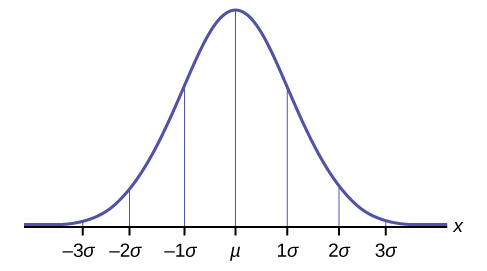
\includegraphics[width=\linewidth]{normal_distribution.jpg}
  \end{column}
 \end{columns}
\end{frame}

\begin{frame}[t]
 \frametitle{Standard Normal Distribution}
 \begin{itemize}
  \item We write $X \sim N(\mu, \sigma)$ to say a random variable $X$ is distributed with a normal distribution with mean $\mu$ and stand deviation $\sigma$.
  \item The \textbf{standard normal distribution} has mean $0$ and standard deviation $1$.
  \item We can change any normal distribution to a standard normal distribution using a \textbf{z-score}.
  $$z = \frac{x - \mu}{\sigma}$$
  \item We can use z-scores to measure standard deviations from the mean
 \end{itemize}
\end{frame}

\begin{frame}[t]
 \frametitle{Example 1}
 \begin{columns}
  \begin{column}{0.5\textwidth}
   Suppose $X \sim N(-1,2)$.
   \begin{itemize}
   \item What is the z-score of $x=2$?
   \item What is the z-score of $x=-13$?
   \item What value is 2 standard deviations to the right of the mean?
   \item What value has a z-score of $-0.5$?
   \end{itemize}
  \end{column}
  \begin{column}{0.5\textwidth}
  \end{column}
 \end{columns}
\end{frame}

\section{The Empirical Rule}

\begin{frame}[t]
 \frametitle{The Empirical Rule}
 \begin{columns}
  \begin{column}{0.5\textwidth}
    \begin{itemize}
     \item About 68\% of the x values lie between $-1\sigma$ and $+1\sigma$ of the mean $\mu$.
     \item About 95\% of the x values lie between $-2\sigma$ and $+2\sigma$ of the mean $\mu$.
     \item About 99.7\% of the x values lie between $-3\sigma$ and $+3\sigma$ of the mean $\mu$.
     \item Notice that almost all the x values lie within three standard deviations of the mean.
    \end{itemize}
  \end{column}
  \begin{column}{0.5\textwidth}
    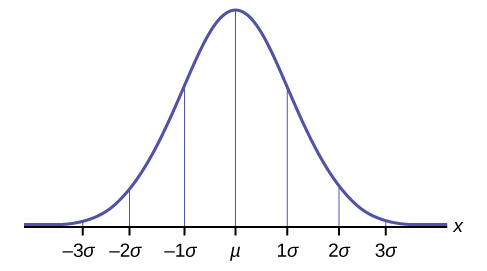
\includegraphics[width=\linewidth]{normal_distribution.jpg}
  \end{column}
 \end{columns}
\end{frame}

\begin{frame}[t]
 \frametitle{Example 2}
 \begin{columns}
  \begin{column}{0.5\textwidth}
   Suppose x has a normal distribution with mean 50 and standard deviation 6. What can we say about the distribution of the data?
  \end{column}
  \begin{column}{0.5\textwidth}
  \end{column}
 \end{columns}
\end{frame}

\begin{frame}[t]
 \frametitle{Example 3}
 \begin{columns}
  \begin{column}{0.5\textwidth}
    From 1984 to 1985, the mean height of 15 to 18-year-old males from Chile was 172.36 cm, and the standard deviation was 6.34 cm.
    \begin{itemize}
     \item About 68\% of the values lie between what two values?
     \item About 95\% of the values lie between what two values?
     \item About 99.7\% of the values lie between what two values?
    \end{itemize}
  \end{column}
  \begin{column}{0.5\textwidth}
  \end{column}
 \end{columns}
\end{frame}

\pagebreak
\section{Using the Normal Distribution}

\begin{frame}[t]
 \frametitle{Using Normal Distributions}
 \begin{columns}
  \begin{column}{0.5\textwidth}
    If $X \sim N(\mu, \sigma)$:
    \begin{itemize}
     \item Calculate $P(X < x)$ by finding the area to the left of $x$ under the bell curve.
     \item Calculate $P(X > x)$ by finding the area to the right of $x$ under the bell curve.
     \item Note: $P(X > x) = 1 - P(X < x)$.
    \end{itemize}
  \end{column}
  \begin{column}{0.5\textwidth}
    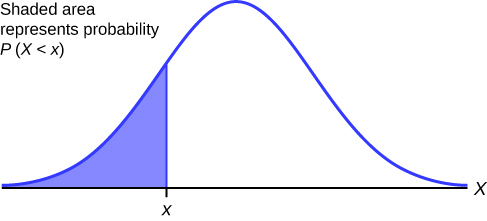
\includegraphics[width=\linewidth]{area_normal_distribution.jpg}
  \end{column}
 \end{columns}
\end{frame}

\begin{frame}[t]
 \frametitle{Calculator Directions}
 To calculate the probability that a normally distributed random variable is between two values:
 \begin{enumerate}
  \item Go to \texttt{Distr -> 2:normalcdf(}.
  \item Enter: lower bound, upper bound, mean, standard deviation.
  \item Type ``)'' and \texttt{Enter}.
 \end{enumerate}
 Note, use ``1 EE 99'' for infinite bounds.

\end{frame}

\begin{frame}[t]
 \frametitle{Example 4}
 \begin{columns}
  \begin{column}{0.5\textwidth}
    The final exam scores in a  class were normally distributed with a mean of 63 and a standard deviation of five.
    \begin{itemize}
     \item Find the probability that a randomly selected student scored more than 65 on the exam.
     \item Find the probability that a randomly selected student scored less than 85 on the exam.
     \item Find the probability that a randomly selected student scored between 58 and 68.
    \end{itemize}
  \end{column}
  \begin{column}{0.5\textwidth}
  \end{column}
 \end{columns}
\end{frame}

\begin{frame}[t]
 \frametitle{Inverse Normal Distribution Function}
 To find the value of $x$ that puts a given area to the left of $x$, use the \texttt{invNorm} function in the \texttt{Distr} menu.
\end{frame}

\begin{frame}[t]
 \frametitle{Example 5}
 \begin{columns}
  \begin{column}{0.5\textwidth}
    The final exam scores in a statistics class were normally distributed with a mean of 63 and a standard deviation of five.
    \begin{itemize}
     \item Find the 70th percentile for the final exam.
     \item Find the 40th percentile for the final exam.
    \end{itemize}
  \end{column}
  \begin{column}{0.5\textwidth}
  \end{column}
 \end{columns}
\end{frame}

\begin{frame}[t]
 \frametitle{Example 6}
 \begin{columns}
  \begin{column}{0.5\textwidth}
    Suppose that the average number of hours a personal computer is used for entertainment is two hours per day and the standard deviation is half an hour.

    \begin{itemize}
     \item Find the probability that a computer is used for entertainment between 1.8 and 2.75 hours per day.
     \item Find the maximum number of hours per day that the bottom quartile of households use a personal computer for entertainment.
    \end{itemize}
  \end{column}
  \begin{column}{0.5\textwidth}
  \end{column}
 \end{columns}
\end{frame}

\end{document}
